\chapter{Examples}

Each example can be installed separately in the workspace using the new wizard.

Choose File > New > Other (or Ctrl-N), open category "eTrice Examples and Tutorials" and select the example you are
interested in. Click Next and Finish and you are ready to go.

Each example comes with the source code generated already. There are also launch configurations for code generation.

\section{Dynamic Actors 1}

This example is contained in \texttt{org.eclipse.etrice.examples.dynamicactors1}.

\subsection{Purpose}

The example demonstrates the usage of an optional actor. It is shown that several actor classes
derived from the type of the optional actor reference can be optionally created in place
of the optional actor reference. Optional actor instances can also be destroyed
and another instance can be created in the free slot.

\subsection{Details}

The structure of this system is simple.

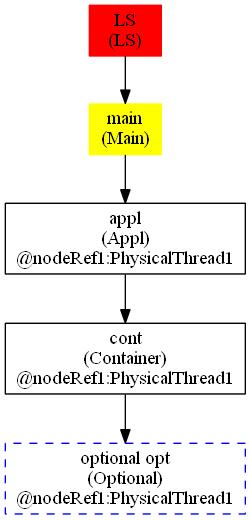
\includegraphics[scale=0.7]{images/039-DynAct1-Main_instanceTree.jpg}

However, this is only the initial system structure.
The leaf instance is just a place holder for an optional actor instance.
In this place an instance of a compatible type can be created at run time.
Compatible types are the type of the reference itself and all of its sub types as long as they are not abstract.
Together with the instance all of its contained instances will be created and all ports are connected.

This example demonstrates how an optional actor is created and destroyed and another one of another type
is created to hold the same place.

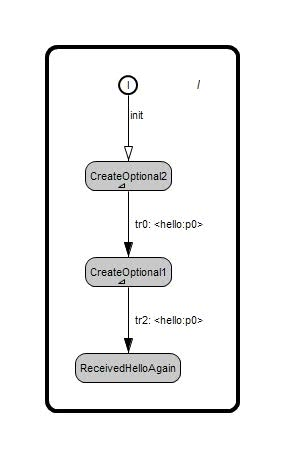
\includegraphics[scale=0.7]{images/039-DynAct1-Container_behavior.jpg}

When the example is executed the \texttt{Container} actor first dumps the instance tree to the console
(line 56 of the listing below).
Then it creates an instance of \texttt{Optional2} (line 57). Now that the \texttt{p0} port
of the container is connected a message \texttt{sayHello()} is sent to the newly created actor instance
and the instance tree is dumped a second time.
As soon as it receives the answer it prints it to the console. Then the optional actor is destroyed again
and another one, now of type \texttt{Optional1}, is created and once more \texttt{sayHello()} is sent.

\lstinputlisting[language=ROOM, firstnumber=36, firstline=36, lastline=73, caption=Container actor state machine]{../../../examples/org.eclipse.etrice.examples.dynamicactors1/model/DynAct1.room}

The console output of the running application starts with

\begin{verbatim}
***   T H E   B E G I N   ***
*** MainComponent /LS/main::init ***
type 'quit' to exit
before creation of Optional2
LS
  main
    RTSystemPort
    MessageService_MessageService_PhysicalThread1
      Dispatcher
      Queue
    ActorClass(className=Appl, instancePath=/LS/main/appl)
      port RTSystemPort
      ActorClass(className=Container, instancePath=/LS/main/appl/cont)
        port RTSystemPort
        port p0
        ScalarOptionalActorInterface(className=Optional, instancePath=/LS/main/appl/cont/opt)
          RTSystemPort
          port p0
    port RTSystemPort0
    port RTSystemPort1
\end{verbatim}

The \texttt{ScalarOptionalActorInterface(className=Optional, instancePath=/LS/main/appl/cont/opt)} is an object which is
responsible for the life cycle of the dynamic actor (including its contained instances) and for the mediation of the
port connections. It contains a replicated \texttt{RTSystemPort} which is used to trigger the initial transition and the
port \texttt{p0} of the interface of the \texttt{Optional} actor class.

After creation of \texttt{Optional2} the interesting part of the dumped tree is

\begin{verbatim}
        ScalarOptionalActorInterface(className=Optional, instancePath=/LS/main/appl/cont/opt)
          RTSystemPort
          port p0
          ActorClass(className=Optional2, instancePath=/LS/main/appl/cont/opt/opt)
            port RTSystemPort
            ActorClass(className=AC2, instancePath=/LS/main/appl/cont/opt/opt/sub2)
              port RTSystemPort
              ActorClass(className=AC3, instancePath=/LS/main/appl/cont/opt/opt/sub2/deep_sub)
                port RTSystemPort
                port p0
          port RTSystemPort0
          port RTSystemPort1
          port RTSystemPort2
\end{verbatim}

It can be seen that the sub tree corresponding to \texttt{Optional2} was inserted right below the
\texttt{ScalarOptionalActorInterface}.

After deletion of the optional actor the dumped instance tree looks exactly as in the beginning.

To illustrate the dynamic behavior of the system we can finally have a look at the generated
sequence diagram \ref{fig:dynact1_msc}. During the sub system initialization three actor
instances are created. Then the system is started and the \texttt{Container} actor dynamically creates
an instance of \texttt{Optional2}. This is indicated by the note on the life line of \texttt{/LS/main/appl/cont}.
Then \texttt{sayHello()} is sent and the answer \texttt{hello()} is received and the optional actor
is destroyed again.

The same is repeated with a new optional instance of \texttt{Optional1}.

\begin{figure}
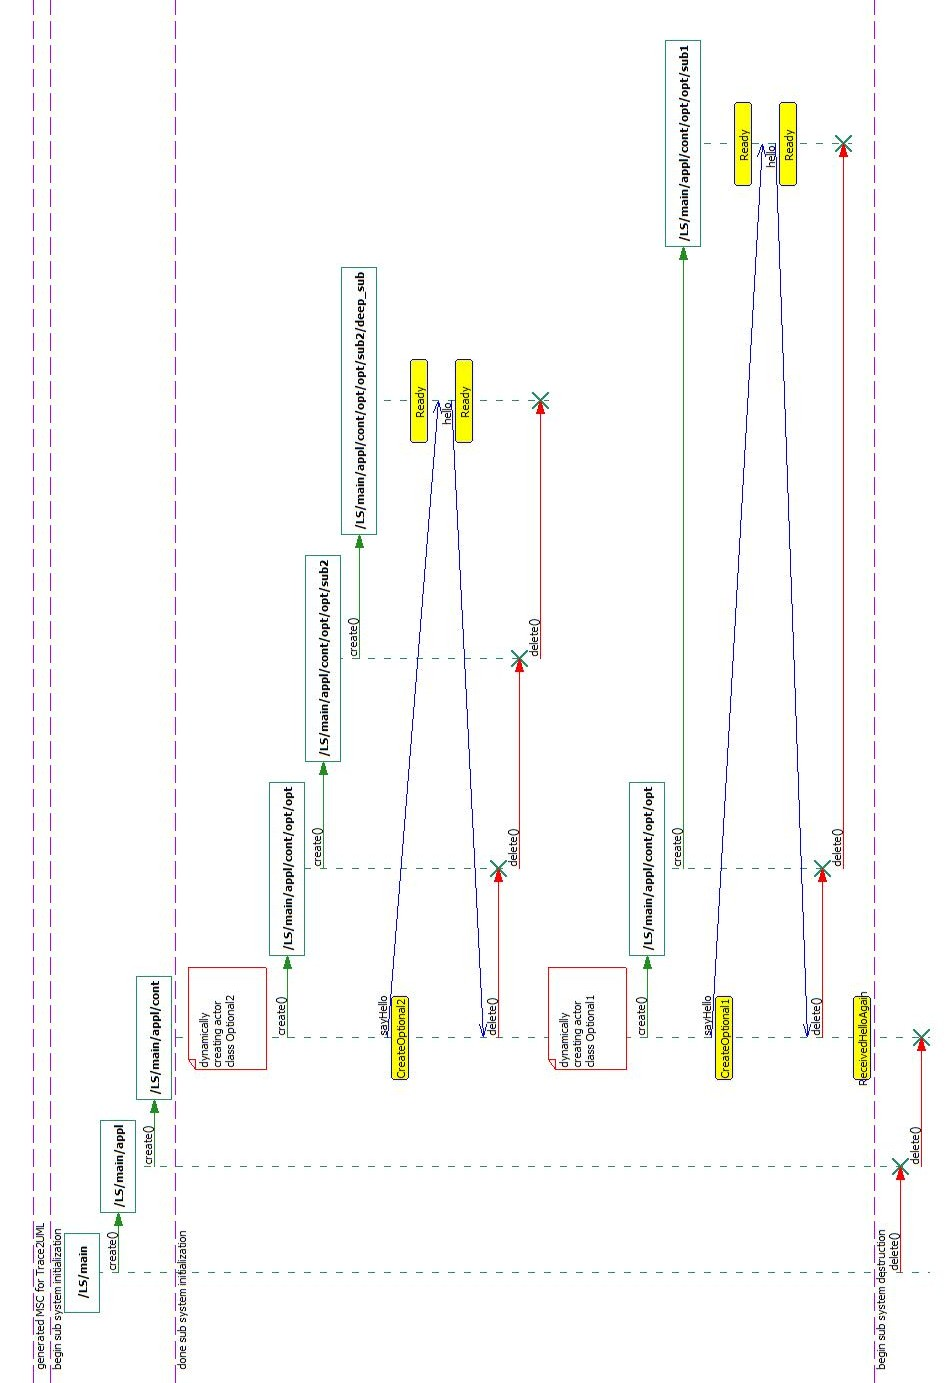
\includegraphics[scale=0.45]{images/039-DynAct1-MSC.jpg}
\caption{Sequence diagram of Dynamic Actors Example 1}
\label{fig:dynact1_msc}
\end{figure}

\subsection{Noteworthy}

\begin{itemize}
\item To obtain an executable the launch configuration \texttt{gen\_DynAct1\_sys.launch} has to be executed.
In this case also the SubsystemClass \texttt{Node\_nodeRef1\_main} is generated as well as factory classes
for the valid optional actors. If \texttt{Optional} were not \texttt{abstract} then also for this class
a factory is created. However, in this class the relay port isn't connected and a request \texttt{sayHello()}
would be left without reply.
\item To generate a library the launch configuration \texttt{gen\_DynAct1.launch} has to be executed.
In this case no factory classes are generated.
\end{itemize}


\section{Dynamic Actors 2}

This example is contained in \texttt{org.eclipse.etrice.examples.dynamicactors2}.

\subsection{Purpose}

A modified version of \texttt{dynamicactors1} is used to analyze eventual memory leaks of the application.

\subsection{Details}

In this modified version creation and deletion of optional actors is looped.
Each loop consists of 4 steps:

\begin{enumerate}
\item create an instance of \texttt{Optional2}
\item destroy the instance
\item create an instance of \texttt{Optional1}
\item destroy the instance
\end{enumerate}

All together 600 steps are performed which corresponds to 300 creations and deletions.

The free memory is printed to the console. Also the overall execution time is measured.
After the loop is finished the heap is analyzed using \texttt{JConsole} (which is a part
of the Java6 distribution) to dump the heap and
\href{http://www.eclipse.org/mat/}{\texttt{org.eclipse.mat}} to analyze it.

The measured total execution time on a Intel Core 2 Duo at 2.66 GHz was 110 ms.
This corresponds to about 370 $\mu$s.

The result of the heap analysis for \texttt{org.eclipse.etrice.*} objects is listed in figure \ref{fig:dynact2_heap}.
The small numbers per object and the retained heap size indicate that the application has no memory leak.

\begin{figure}
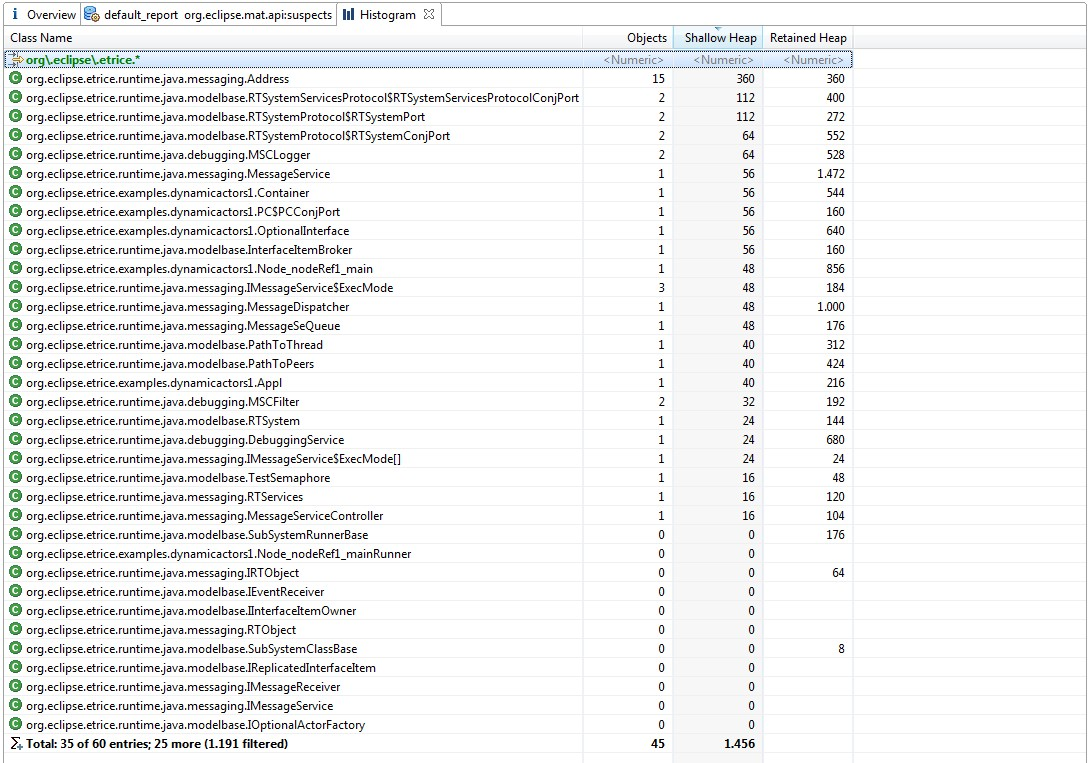
\includegraphics[scale=0.45]{images/039-DynAct2-HeapAnalysis.jpg}
\caption{Heap analysis after 600 steps}
\label{fig:dynact2_heap}
\end{figure}

\subsection{Noteworthy}

\begin{itemize}
\item Calling the garbage collector every time before the free memory is dumped
costs a significant amount of time and the execution time is increased to the order of seconds.
\item The measured free memory is close to constant. Only a small step is observed which wasn't analyzed further.
\end{itemize}

\section{Dynamic Actors 3}

This example is contained in \texttt{org.eclipse.etrice.examples.dynamicactors3}.

\subsection{Purpose}

The example demonstrates the usage of an optional actor array. It is shown that several actor classes
derived from the type of the optional actor reference can be created as array members.
The array members can be destroyed in arbitrary order and the array size grows and shrinks as appropriate.

\subsection{Details}

This example again is similar to example 1. One difference is that the (scalar) optional actor is replaced by a
replicated optional actor (or array of optional actors if you wish).
The port of the \texttt{Container} was also changed to a replicated port. All replication factors in this example
are of arbitrary multiplicity (*). The sizes vary dynamically and are unbound as far as the model is concerned.

The behavior was changed to the following:
Two instances of different classes are created as members of this array and both are deleted and one is created again.
The replicated port is used to send (broadcast) messages to the optional actors.

\subsection{Noteworthy}

\begin{itemize}
\item the generated MSC \texttt{main\_Async.seq} is a good illustration of the dynamic changes in the system structure
\item careful inspection of the console output reveals that objects are created and destroyed as expected
\end{itemize}

\section{Dynamic Actors 4}

This example is contained in \texttt{org.eclipse.etrice.examples.dynamicactors4}.

\subsection{Purpose}

The example demonstrates the usage of an optional actor. But here not the actor containing the optional reference
is communicating with the optional actor but one level above.

\subsection{Details}

The \texttt{Controller} which has a reference to the \texttt{Container} is asking the latter
for the creation of the dynamic actor. When it receives \texttt{ok()} it is requesting \texttt{sayHello()}
from the newly created actor.

After the \texttt{Controller} receives \texttt{hello()} it tells the \texttt{Container} to create another
actor which fails because the old one is still in place.

\subsection{Noteworthy}

\begin{itemize}
\item the generated MSC \texttt{main\_Async.seq} is a good illustration of the dynamic changes in the system structure
\end{itemize}

\section{Dynamic Actors 5}

This example is contained in \texttt{org.eclipse.etrice.examples.dynamicactors5}.

\subsection{Purpose}

The example shows that the optional actor can not only have relay ports but also external end ports.

\subsection{Details}

This simple example just shows that the optional actor may directly handle inbound messages by using an
external end port rather than the relay port of the previous examples.

\subsection{Noteworthy}

\begin{itemize}
\item the generated MSC \texttt{main\_Async.seq} is a good illustration of the dynamic changes in the system structure
\end{itemize}

\section{Dynamic Actors 6}

This example is contained in \texttt{org.eclipse.etrice.examples.dynamicactors6}.

\subsection{Purpose}

The example demonstrates the use of nested dynamic actors.

\subsection{Details}

In this example the dynamically created actor \texttt{Optional2} has again an optional reference two levels down in its hierarchy.
On creation it immediately creates a nested dynamic actor of class \texttt{Optional1} which is sending \texttt{hello()} back
to the outer \texttt{Container}.

\subsection{Noteworthy}

\begin{itemize}
\item the generated MSC \texttt{main\_Async.seq} is a good illustration of the dynamic changes in the system structure
\item when a dynamic actor is created its structure is there immediately and all ports are connected. But the initial transition
is executed asynchronously. So after the outer dynamic actor is created the port of the \texttt{Container} is not yet connected
because the initial transition which is responsible for the creation of the inner dynamic actor wasn't executed yet.
So a message sent from this port directly after creation of the outer dynamic actor would get lost.
\end{itemize}
